% \documentclass[11pt,a4paper]{scrartcl}
\documentclass[twoside,10pt,a4paper]{article}
\setlength{\parindent}{0em}
\setlength{\parskip}{1.5em}


\renewcommand{\familydefault}{\sfdefault}

\newenvironment{notes}[1][\unskip]{%
\par
\noindent
\textcolor{blue}{\bfseries{Notes - } #1:}
\\ \color{blue}}
{}

\newenvironment{followup}[1][\unskip]{%
\par
\noindent
\textcolor{red}{\bfseries{Follow-up - } #1!!!}
\\ \color{red}}
{}

\newenvironment{question}[1][\unskip]{%
\par
\noindent
\textcolor{orange}{\bfseries{Question - } #1???}
\\ \color{orange}}
{}

\usepackage{mystyle}
% Document Layout
% ---> Document geometry - current setting is set to A4 with relatively narrow margins
\geometry{
  a4paper,
  total={210mm,297mm}, % A4 paper measurement
  left=20mm,
  right=20mm,
  top=25mm,
  bottom=25mm
  }
% ---> Document header and footer setting
\pagestyle{fancy}
\fancyhead[LE,RO]{\leftmark} % Refer to Section/chapter/part on the upperroght of the heading
\fancyhead[RE,LO]{}
\fancyfoot[CE,CO]{}
\fancyfoot[LE,RO]{Page \thepage \, of \pageref{LastPage}} % Print current page and total page number centered in the footer.
% ---> Header and footer horisontal line borders
\renewcommand{\headrulewidth}{1pt}
\renewcommand{\footrulewidth}{0.5pt}

% \definecolor{cell-lghtGry}{RGB}{200,200,200}

% Typesetting code snippets
% The code snippet typesetting below is based on https://www.latextemplates.com/template/code-snippet
% Original Author: This template was created for LaTeXTemplates.com by vel@latextemplates.com
\definecolor{DarkGreen}{rgb}{0.0,0.4,0.0} % Comment color
\definecolor{highlight}{RGB}{204,255,229} % Code highlight color
\definecolor{Gray}{RGB}{224,224,224}
\definecolor{Purple}{RGB}{255,0,255}
\definecolor{Blue}{RGB}{0,0,255}

\lstdefinestyle{Style1}{ % Define a style for your code snippet, multiple definitions can be made if, for example, you wish to insert multiple code snippets using different programming languages into one document
language=Perl, % Detects keywords, comments, strings, functions, etc for the language specified
backgroundcolor=\color{highlight}, % Set the background color for the snippet - useful for highlighting
basicstyle=\footnotesize\ttfamily, % The default font size and style of the code
breakatwhitespace=false, % If true, only allows line breaks at white space
breaklines=true, % Automatic line breaking (prevents code from protruding outside the box)
captionpos=b, % Sets the caption position: b for bottom; t for top
commentstyle=\usefont{T1}{pcr}{m}{sl}\color{DarkGreen}, % Style of comments within the code - dark green courier font
deletekeywords={}, % If you want to delete any keywords from the current language separate them by commas
%escapeinside={\%}, % This allows you to escape to LaTeX using the character in the bracket
firstnumber=1, % Line numbers begin at line 1
frame=single, % Frame around the code box, value can be: none, leftline, topline, bottomline, lines, single, shadowbox
frameround=tttt, % Rounds the corners of the frame for the top left, top right, bottom left and bottom right positions
keywordstyle=\color{Blue}\bf, % Functions are bold and blue
morekeywords={}, % Add any functions no included by default here separated by commas
numbers=left, % Location of line numbers, can take the values of: none, left, right
numbersep=10pt, % Distance of line numbers from the code box
numberstyle=\tiny\color{Gray}, % Style used for line numbers
rulecolor=\color{black}, % Frame border color
showstringspaces=false, % Don't put marks in string spaces
showtabs=false, % Display tabs in the code as lines
stepnumber=5, % The step distance between line numbers, i.e. how often will lines be numbered
stringstyle=\color{Purple}, % Strings are purple
tabsize=2, % Number of spaces per tab in the code
}

% Create a command to cleanly insert a snippet with the style above anywhere in the document
\newcommand{\insertcode}[2]{\begin{itemize}\item[]\lstinputlisting[caption=#2,label=#1,style=Style1]{#1}\end{itemize}} % The first argument is the script location/filename and the second is a caption for the listing

% Enable indexing and create an index with following formating
\makeindex[columns=4, title=Index, intoc]

\pagenumbering{roman}

\begin{document}

  % title ans pharagraps section
  \begin{titlepage}

  \begin{center}

    \textcolor{red}{\Huge{THIS IS AN EMPTY TITLE-PAGE TEMPLATE}} % Remove or comment out this line.


      {\bfseries{\Huge{Reflective Journal}}}


      {\Large{by}}

    \begin{author}
      \author{\Large{Insert author name}}
    \end{author}


    \vspace*{2.5cm}
    Submitted for Assessment in


    \begin{title}
        \title{\bfseries{\huge{Insert Title}}}
    \end{title}

    \vspace*{2.5cm}
    at


    \Large{Noroff University Collegge}

    \vfill


    \begin{figure}[h!]
      \centering
      
\includegraphics[height=50pt]{Noroff-Logo.png}
    \end{figure}


  \end{center}
\end{titlepage}

  
  % \frontmatter
  % front page, title, table of content etc. will have separate page numbering.
  \tableofcontents
  
  \newpage

  % \listoffigures % uncomment to create list of figures
  % \listoftables % uncomment to create list of tables

  % main document will be rendered with the files listed in this section
  % \mainmatter

  \newpage
  \section{Introduction}

% Remove or comment out this whole environment when using this template.
{\begin{center}
    \textcolor{red}{\Huge{THIS IS A SAMPLE INTRODUCTION SECTION}}

    \begin{tabular}{r @{: } p{80mm}}
        {\textcolor{blue}{Blue text}} &  Help text. Short description of how to use an environment or a section in the template.\\
        <<text placeholder>> & Text between angle brackets are placeholders. Indicates a string to be replaced with input text.\\
        Normal text/black fonts & Real note/example text, how the section is intended to be used.
    \end{tabular}

\end{center}


{\huge{Course: <<course code>> <<course name>>}}

<<course moodle path>>

\subsection{Key dates}

\begin{tabular}{r @{ : } c}
    Duration: & 6 weeks\\
    Start & 1900-01-01\\
    End & 1900-01-01\\
    Formative assessment & TBD\\
    Assessment 1 - Submission date & TBD\\
    Assessment 2 - Submission date & TBD\\
\end{tabular}

\subsection{Course Tutors}

\begin{tabular}{r @{ : } l}
    Course leader & Arthur Dent\\
    Course lecturer & Ford Prefect\\
    Course tutor & John Crichton\\
    course tutor & Aeryn Sun\\
    Support tutor & Ka D'Argo\\
    Support tutor & Chiana\\
    Support tutor& Rygel\\
    Support tutor & Pa'u Zotoh Zhaan\\
\end{tabular}

\subsection{Study goals}

\begin{itemize}
    \item Working with database (SQLite)
        \begin{itemize}
            \item Find Moya
            \item Escape from Scorpius
            \item Feed Rygel
            \item Save the galaxy
        \end{itemize}


\end{itemize}


  \newpage
  \pagenumbering{arabic}
  \setcounter{page}{1}
  % This is a section template for reflective journal

% Remove or comment out this whole environment when using this template.
{\begin{center}
    \textcolor{red}{\Huge{THIS IS A FILLED SAMPLE SECTION}\\[4mm] ...with realistic notes...}

    \begin{tabular}{r @{: } p{80mm}}
        {\textcolor{blue}{Blue text}} &  Help text. Short description of how to use an environment or a section in the template.\\
        <<{\emph{text placeholder}}>> & Text between angle brackets are placeholders. Indicates a string to be replaced with input text.\\
        Normal text/black fonts & Real note/example text, how the section is intended to be used.
    \end{tabular}

\end{center}

% ----> Header informaton section - Start
\section{Lesson 1: Course Introduction}

Original URL: \url{https://www.noroff.no}
% <---- Header informaton - End


% ----> Main reflective subsection - Start
% ----| Write reflective thoughts on the topic in general. |----
\subsection{Reflection on the days lecture and tutorial}

Lesson 1 was an introduction on the subject of {\emph{Programming Databases}}. It gave a nice overview about the subject, how it is layed out, and perhaps most importantly the study goal. Compared to the 3 other subjects taken since the start of this course, it is the first subject where the subject was clearly outlined along with the goals.

There was a statement, see quote on page \pageref{quote} from Prof. Johan Van Niekerk, which is important to keep in the back of mind. It should perhaps be pinned to the wall as a reminder of a pitfall to be cognizant of when surmounting challenging study phases. A reminder to wisely allocate the effort exerted, and lower the level of pondering on the vastness of relevant topics, but stay in focus inside the subject domain, at hand.

The statement resonated with me personally, since I regard lack of focus and wasted effort as one culprit of my struggle to keep up on course materials and assessments. I find it very easy to veer of on a tangent and wander away from the study material. For example, making search queries and delving into statistics, while addressing probability in discrete math.

% <---- Main reflective subsection - End



% ----> Main reflective subsection - Start
% ----| Write reflective thoughts on a specific reflective topic. |----
\subsection{Reflection Topics}

None applicable for this lesson. No reflection topics given for this lesson.

% <---- Main reflective subsection - End



% ----> Key Take-Away subsection - Start
% ----| Write Itemized notes regarding the lesson topic. |----
\subsection{Key Take-Away}

Items/bullet points outlines  below outlines key information from the day's lesson.

\begin{itemize}
    \item Working with database (SQLite)
        \begin{itemize}
            \item Acquire fundamental skill about working with databases
            \item How to design as simple normalized database
            \item Understand database storage and data structure
            \item Understand database Normalization
            \item Be able to query and interface with databases
            \item How to script and automate database connection, mangagement and datamining
            \item Automate data manipulation and analysis, generating reports and statitics etc on data in databases, dataframes etc.
            \item Understanding and being able to manage and  work with databases is therefore key to the field of CyberSecurity.
        \end{itemize}
\end{itemize}

Course: UC1PR2101 - Programming Databases

\begin{enumerate}
    \item New lesson structure.
        \begin{enumerate}
            \item The course is layed out to be taken with a more individual approach, akin to remote studies. More preparation are expected prior to lecture sessions.
            \item Lessons are broken up into smaller topics.
            \item Reflective Journals are not mandated. 20\% of the mark will not be allocated to Reflective Journal submition.
            \item Quizes will be smaller and with a formative purpose. There will be a practice Quizes.
            \item Overall reduced number of submition for assessment. Course grades will be based on 1 or 2 larger assessments, instead of many smaller assessments.
            \item Course assessment targets, along with target dates to be posted soon.
        \end{enumerate}
    \item New Lecture structure.
        \begin{enumerate}
            \item Students are expected to engage with study material at least 1 day ahead.
            \item Students are expected to be more prepared for each lecture topics.
            \item Referenced resources are not "mandatory", students must choose what materials are applicable and important.
        \end{enumerate}
    \item Tools and applications
        \begin{enumerate}
            \item SQLite
            \item Python
            \item PANDAS(?)
        \end{enumerate}
\end{enumerate}

Learning Databases itself is a comprehensive part of software engineering and software development, which cannot be condensed in a 6 week course.

\begin{displayquote}\label{quote}
    {\emph{We are not software developers. Our purpose is to learn enough to be able to understand enough to know what we are looking at when we are working with someone elses (database) design templates...\\}}
    {\ttfamily{
        - Prof. Johan Van Niekerk}}
\end{displayquote}

Analogous to learning enough foriegn language; One is not expected to be a fluent speaker. But know enough, to converse and to be able to accomplish a specific goal. Deeper knowledge are obtained along the way, where fluency comes through effort and immersion over time. 

My personal take on this (to make it relatable to the course) is as follows: A car crash forrensic investigator should know enough about a car to tell the pieces from eachother, but is not expected to fix, design or engineer a car to prodution.

% <---- Key Take-Away subsection - End


% ----> Lessons Learned subsection - Start
% ----| Write a summary about the day's lesson topic. |----
\subsection{Lessons Learned}

This subsection summarizes the day's lesson topic.

\begin{itemize}
    \item Why databases (in relation to CyberSecurity)?
        \begin{itemize}
            \item Acquire fundamental skills about the purpose of databases
            \item Understand how databases are key to modern data and information infrasctructure
            \item Get an overview of the majority of todays transactional databases today and their use of relational database
            \item Understand how systems and data breach are on the database connectivity and transactional level
        \end{itemize}
    \item What is a database?
        \begin{itemize}
            \item Acquire fundamental skills about what a database is
            \item What databases are used for
            \item What types of databases are in use
        \end{itemize}
    \item Where does database fit into the ecosystem of "data"?
        \begin{itemize}
            \item Be able to identify different ways of storing, structuring and organizing data.
        \end{itemize}
\end{itemize}


{\bfseries{Databases}}

Databases organize data/information by following examples.

\begin{itemize}
    \item Catagorization
    \item Quantify
    \item Itemization
    \item Relation etc.
\end{itemize}

Database systems aims to resolve some data storage issues such as problemetic {\emph{Data redundancy/duplication}}:
\begin{itemize}
    \item Storage, takes space
    \item Overhead, when updating
    \item Itegrity, data consistency
\end{itemize}

{\bfseries{Glossary:}}

\begin{tabular}{p{40mm} | p{120mm}}
    {\bfseries{Key Word/Expression}} & {\bfseries{Elaboration/Comment}}\\ \hline
    Database & A logical way to organize, store, label and describe relationships of data.\\ \hline
    Third Normal Form & Relational databases. A database schema design see "Other source material" table in section \ref{subsec:source}. Ensures update and insert integrity to the database.\\ \hline
    (Working in) Disconnected mode & A safe way to work with data in Databases, to avoid data curruption or data integrity error. Such curruption or error can occur when multiple connections are made and edits the same data at the same time. Tracking which changes, by which connections, is the most recent and valid change will be difficult. Working in "Disconnected Mode" will remedy this issue.\\ \hline
    SQL & {\bfseries{S}}tructured {\bfseries{Q}}uery {\bfseries{L}}anguage - a standardized language to interface with databases\\ \hline
    DDL & {\bfseries{D}}ata {\bfseries{D}}efinition {\bfseries{L}}anguage - tells a database how it data will be stored or organized. \\ \hline
    DML & {\bfseries{D}}ata {\bfseries{M}}anipulation {\bfseries{L}}anguage - tells the database how to operate the data. \\ \hline
    Database Normalization & Structuring a relational database, reduce data duplication and improve data integrity. \\ \hline
\end{tabular}

\begin{figure}
    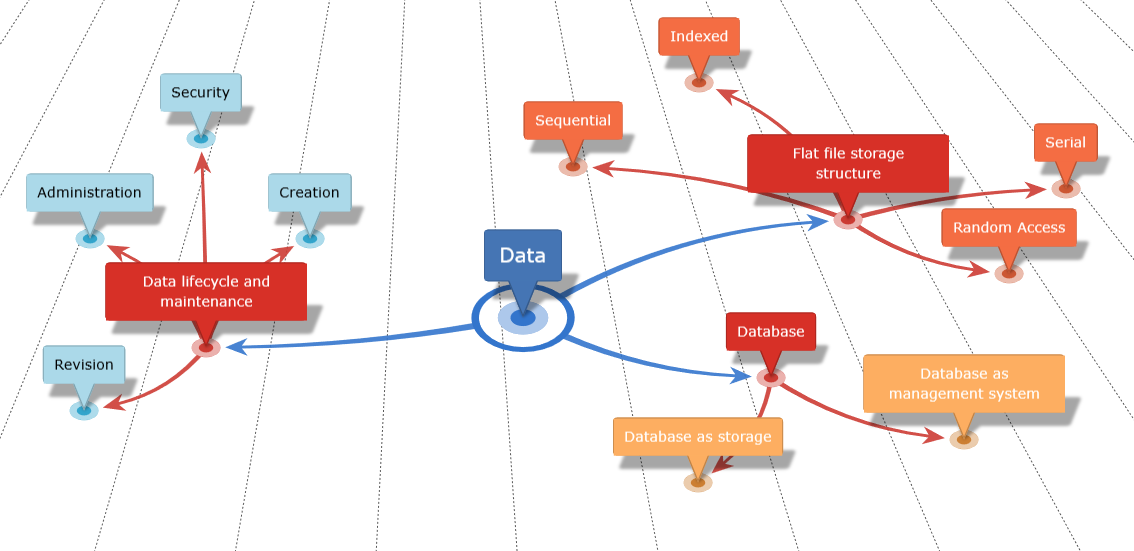
\includegraphics[width=\linewidth]{tex/Data_cropped.png}
    \caption{Data Mindmap}
    \label{fig: Data Mindmap}
\end{figure}

\begin{figure}
    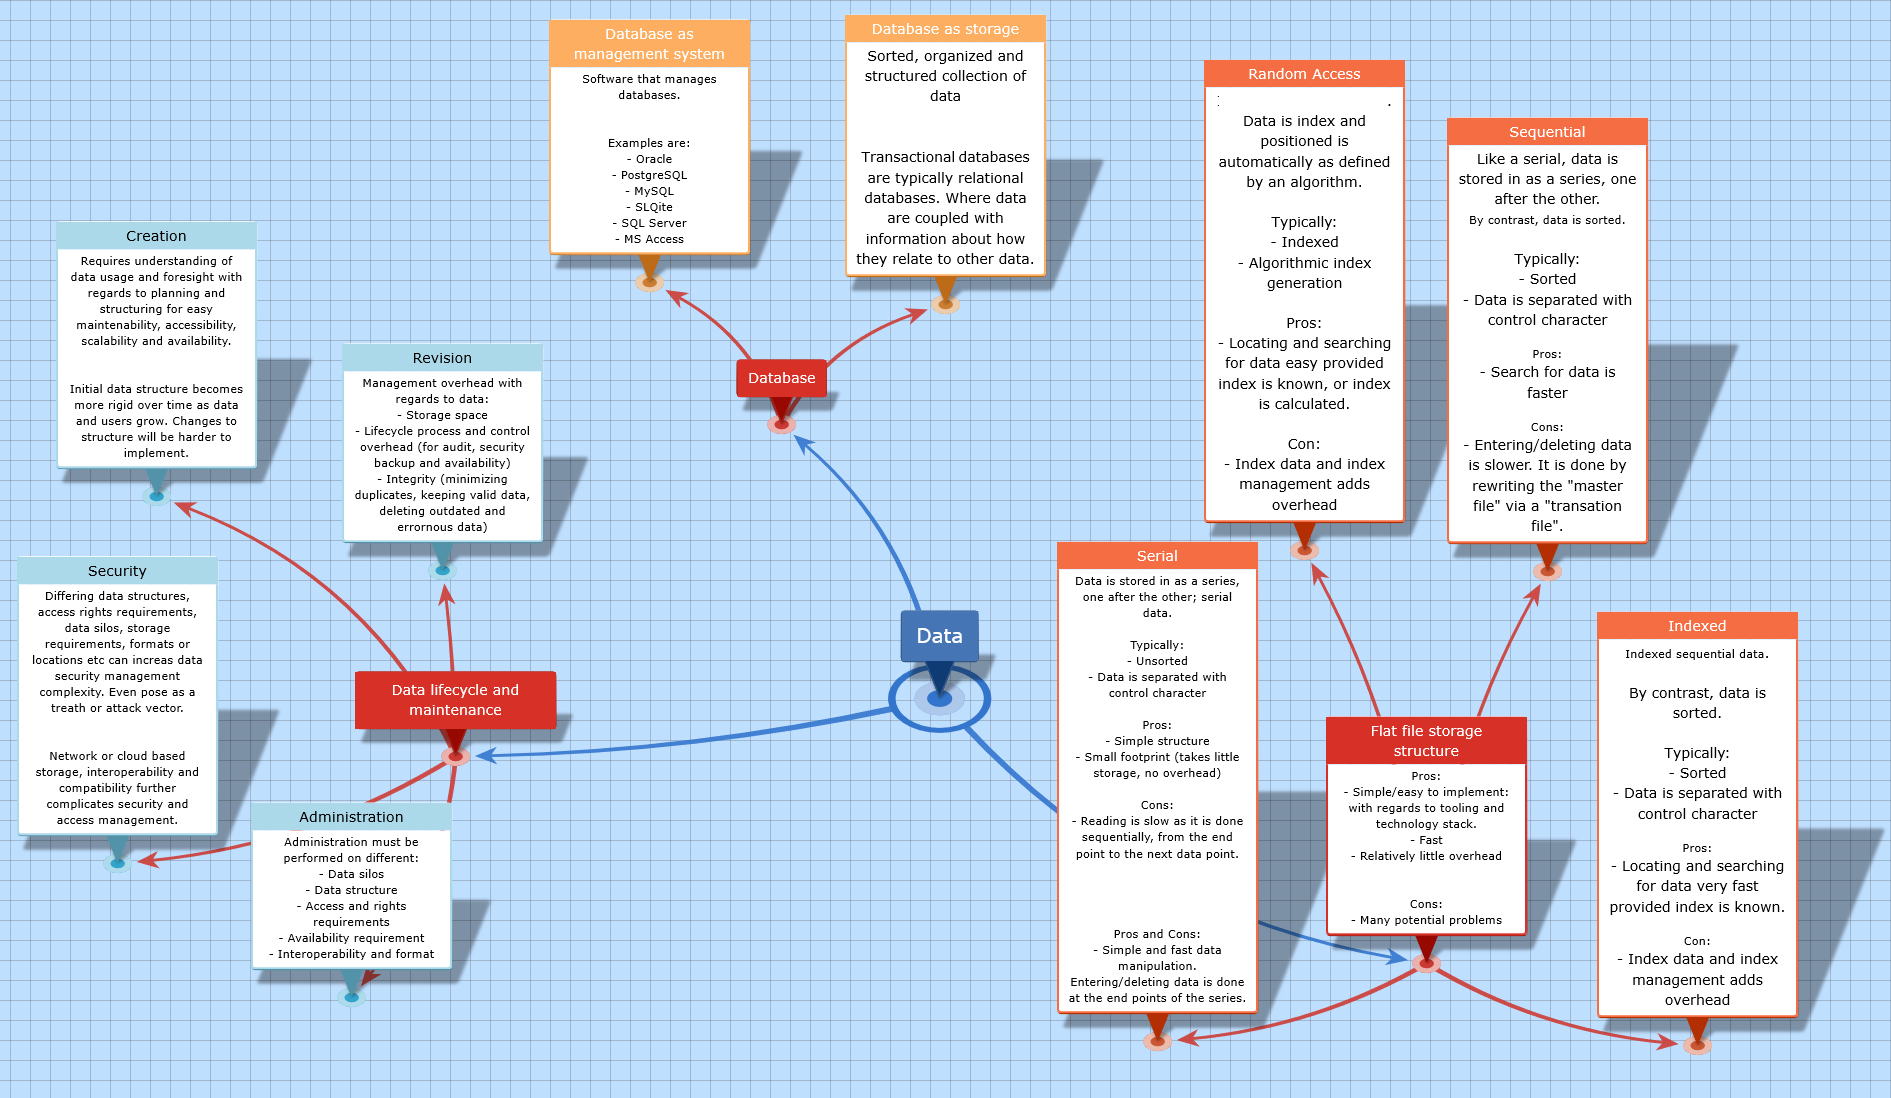
\includegraphics[width=\linewidth]{tex/Data_cropped2.png}
    \caption{Data Mindmap - with detailed notes expanded}
    \label{fig:Data Mindmap expanded}
\end{figure}

% <---- Lessons Learned subsection - End


% ----> Action-Point subsection - Start
% ----| To-do list to complete the day's lesson topic. |----
\subsection{Action Points - Further Reading/Enquiry}

\begin{adjustbox}{max width=\textwidth}
    \begin{tabular}{c|l|l|c|l}
        {\bfseries{Action Point}} & {\bfseries{To-do description}} & {\bfseries{Assigned to}} & {\bfseries{Target date}} & {\bfseries{Comment/Status}} \\
        \hline
        1 & Verify/enroll to Teams channel membership for the course & N/A & ASAP & Assigned \\ \hline
        2 & Setup a home-lab with SQLite & N/A & ASAP & Assigned \\ \hline
        3 & Look up and learn SQL (DDL, DML etc) & N/A & ASAP & Assigned \\ \hline
        4 & Look up and learn UML & N/A & ASAP & Assigned \\ \hline
    \end{tabular}
\end{adjustbox}

% <---- Action-Point subsection - End



% ----> Other source materials subsection - Start
% ----| A list of materials not directly provided via the course books/distributed by lecturers for the day's lesson topic. |----
\subsection{Other source materials} \label{subsec:source}

\begin{tabular}{p{40mm} | p{120mm}}
    {\bfseries{Resource Type}} & {\bfseries{Source description, Book title, URL, etc.}}\\
    \hline
    Wikipedia - 3rd Normal Form & \url{https://en.wikipedia.org/wiki/Third_normal_form}\\ \hline
    Wikipedia - SQLite & \url{https://en.wikipedia.org/wiki/SQLite}\\ \hline
    Youtube - SQLite & \url{https://www.youtube.com/watch?v=byHcYRpMgI4}\\ \hline
    YouTube - SQLite usecases & \url{https://www.youtube.com/watch?v=Jib2AmRb_rk}\\ \hline
    SQLite - Official & \url{https://sqlite.org/index.html}\\ \hline
\end{tabular}

% <---- Other source materials subsection - end


% ----> Issues Noted and Area of Improvements subsection - Start
% ----| A list of items, after-thought about issues, difficulties (on the subject itself, materials, tools, etc.) working with the day's lesson topic. |----
\subsection{Issues Noted and Area of Improvements}

\begin{tabular}{c|l}
    {\bfseries{Issue number}} & {\bfseries{Issue description / Area of Improvement}}\\
    \hline
    1 & N/A\\ \hline
    2 & N/A\\ \hline
    
\end{tabular}


% <---- Issues Noted and Area of Improvements subsection - End
  
  
  \newpage
  % This is a section template for reflective journal


% Remove or comment out this whole environment when using this template.
{\begin{center}
    \textcolor{red}{\Huge{THIS IS AN EMPTY SECTION TEMPLATE}}

    \begin{tabular}{r @{: } p{80mm}}
        {\textcolor{blue}{Blue text}} &  Help text. Short description of how to use an environment or a section in the template.\\
        <<{\emph{text placeholder}}>> & Text between angle brackets are placeholders. Indicates a string to be replaced with input text.\\
        Normal text/black fonts & Real note/example text, how the section is intended to be used.
    \end{tabular}

\end{center}


% ----> Header informaton section - Start
\section{Lesson <<{\emph{number}}>>: <<{\emph{Lesson topic}}>>}

{\textcolor{blue}{Replace the double angle brackets with the lesson number and name.}}

Original URL: <<{\emph{link to the original blog post on the Moodle blog}}>>

{\textcolor{blue}{Replace the double angle brackets with the URL to the reflective journal blog.}}
% <---- Header informaton - End


% ----> Main reflective subsection - Start
% ----| Write reflective thoughts on the topic in general. |----
\subsection{Reflection on the days lecture and tutorial}

{\textcolor{blue}{In the list below, specify lesson topics and goals. Describe how the topics will be approached.}}

{\bfseries{Lesson/Topic Objectives \& Study Plan:}}
\begin{itemize}
    \item Topic 1 - 1 day lecture
    \item Topic 2 - 2 day lecture + lab and tests
    \item Topic 3 - 2 day lecture
\end{itemize}

A groups project covering all topics to be submitted by the end of lecture}

{\textcolor{blue}{Add critical reflective thoughts about your learning experiences. Delete this text}}


% <---- Main reflective subsection - End

% ----> Main reflective subsection - Start
% ----| Write reflective thoughts on a specific reflective topic. |----
\subsection{Reflection Topics}

{\textcolor{blue}{When there are guided topics add them as sub-headings and include your critical discussion of the topic(s)}}

<<{\emph{\blindtext[1]}}>> % Example text, comment out or remove this line.

<<{\emph{\blindtext[1]}}>> % Example text, comment out or remove this line.

\subsubsection{Provided topic 1}

{\textcolor{blue}{topic 1 example reflective discussion}}

<<{\emph{\blindtext[1]}}>> % Example text, comment out or remove this line.

<<{\emph{\blindtext[1]}}>> % Example text, comment out or remove this line.

\subsubsection{Provided topic 2}

{\textcolor{blue}{topic 2 example reflective discussion}}

% <---- Main reflective subsection - End



% ----> Key Take-Away subsection - Start
% ----| Write Itemized notes regarding the lesson topic. |----
\subsection{Key Take-Away}

\begin{table}[H]
    \begin{tabular}{p {20mm} @{: } p{80mm}}
        Lesson date & {\emph{<<yyyy mm dd>>}} \\
        Date taken & {\emph{<<yyyy mm dd>>}} \\
        Revisited & <<{\emph{comment or yyyy mm dd}}>> \\
    \end{tabular}
\end{table}

{\textcolor{blue}{This subsection outlines key information from the day's lesson in bullet points.}}

\begin{enumerate}\itshape
    \item <<Main Item 1
    \begin{enumerate}
        \item sub item 1 1
        \item sub item 1 2
        \item sub item 1 3
        \item sub item 1 4
        \item sub item 1 5
        \item sub item 1 6
    \end{enumerate}
    \item Main Item 2
    \begin{enumerate}
        \item sub item 2 1
        \item sub item 2 2
        \item sub item 2 3
        \item sub item 2 4
    \end{enumerate}
    \item Main Item 3
    \item ..
    \item .>>
\end{enumerate}


\subsection{Lessons Learned}

{\textcolor{blue}{This subsection summarizes the day's lesson topic.}}

{\bfseries{Bold heading}}

<<{\emph{\blindtext[2]}}>>


{\bfseries{Glossary:}}

{\textcolor{blue}{Expand and elaborate on new words, expressions and topic terminology with a glossary list.}}

\begin{table}[H]\label{tab:glossary}
    \begin{tabular}{p{40mm} | p{120mm}}
        {\bfseries{Key Word/Expression}} & {\bfseries{Elaboration/Comment}}\\ \hline
        <<{\emph{Input}}>> & <<{\emph{Input}}>>\\ \hline
    \end{tabular}
\end{table}

% <---- Lessons Learned subsection - End



% ----> Action-Point subsection - Start
% ----| To-do list to complete the day's lesson topic. |----
\subsection{Action Points - Further Reading/Enquiry}

{\textcolor{blue}{To-do list relevant to complete/expand on the lesson topic.}}

\begin{adjustbox}{max width=\textwidth}
    \begin{tabular}{c|l|l|c|l}
        {\bfseries{Act Pnt}} & {\bfseries{To-do description}} & {\bfseries{Assigned to}} & {\bfseries{Target date}} & {\bfseries{Comment/Status}} \\
        \hline
        1 & <<{\emph{Task name/description}}>> & <<{\emph{Task owner}}>> & <<{\emph{Deadline yyyy-mmm-dd}}>> & <<{\emph{Comments or status}}>> \\ \hline
        2 & <<{\emph{Task name/description}}>> & <<{\emph{Task owner}}>> & <<{\emph{Deadline yyyy-mmm-dd}}>> & <<{\emph{Comments or status}}>> \\ \hline
    \end{tabular}
\end{adjustbox}

% <---- Action-Point subsection - End



% ----> Other source materials subsection - Start
% ----| A list of materials not directly provided via the course books/distributed by lecturers for the day's lesson topic. |----
\subsection{Other source materials} 

{\textcolor{blue}{External course related material. Insert book title, ISBN, URL etc. }}

\begin{table}[H]\label{tab:sources}
    \begin{tabular}{p{10mm} | p {47mm} | p{100mm}}
        {\bfseries{Item num.}} & {\bfseries{Resource Type}} & {\bfseries{Source description, Book title, URL, etc.}}\\
        \hline
        1 & <<{\emph{Input}}>> & <<{\emph{Input}}>>\\ \hline
    \end{tabular}
\end{table}

% <---- Other source materials subsection - end

% ----> Issues Noted and Area of Improvements subsection - Start
% ----| A list of items, after-thought about issues, difficulties (on the subject itself, materials, tools, etc.) working with the day's lesson topic. |----
\subsection{Issues/Solutions Noted and Area of Improvements}

{\textcolor{blue}{Issues noted; what has failed with regards to tools, the lecture itself, missing course material, wrong information or solution in the course assignment etc. Any area of improvement with regards to how previous task has been managed, how to more efficiently proceed with the course personally. Suggestions for improvement suggestions to course leader.}}

\begin{table}[H]\label{tab:issuensolution}
    \begin{tabular}{p{10mm} | p {47mm} | p{100mm}}
        {\bfseries{Item num.}} & {\bfseries{Issue description / Area of Improvement}} & Comments / Solution \\ \hline
        1 & <<{\emph{input}}>> & <<{\emph{input}}>>\\ \hline
    \end{tabular}
\end{table}

% <---- Issues Noted and Area of Improvements subsection - End
  
  
  \newpage
  \section{This is body\_section3 heading}

{\begin{center}
    \textcolor{red}{\Huge{THIS IS AN EMPTY SAMPLE SECTION}\\[4mm] ...single page, no subsections...}

    \begin{tabular}{r @{: } p{80mm}}
        {\textcolor{blue}{Blue text}} &  Help text. Short description of how to use an environment or a section in the template.\\
        <<{\emph{text placeholder}}>> & Text between angle brackets are placeholders. Indicates a string to be replaced with input text.\\
        Normal text/black fonts & Real note/example text, how the section is intended to be used.
    \end{tabular}

\end{center}

<<{\emph{\blindtext[2]}}>>

  

  \newpage
  \section{This is body\_section4 heading}


\blindtext[3]


\subsection{Sub Test}
This is a pharagraph


\subsubsection{Sub Sub Test}
This is a pharagraph


\blindtext[5]


\blindtext[3]


\blindtext[3]
  
  
  \newpage
  \section{Conclusion}

Conclusion

\insertcode{tex/hello_world.py}{This is "Hello World" in Python}

This is the conclusion page with a code listing.

\blindtext[2]


  \newpage
  \appendix
  \section{Appendix}

This is the appendix

  % bibliography
  \clearpage
  \section{Bibliography}

Bibliography

  \newpage
  \printindex
  
\end{document}